\chapter{Analyse du code}

Notre projet s'effectue dans la continuité d'un projet déjà bien entamé, ainsi, la première étape est de comprendre et d'assimiler le travail qui a déjà été effectué. Le fait que nous codons par dessus un code qui n'est pas le nôtre nous a compliqué la tâche lors de l'implémentation de certaines fonctions, comme l'intégrateur. L'analyse du code consistera en une description de chaque fichier et des structures utilisées, le code est très commenté.

\section{Visualisation}
L'affichage est géré par les fichiers \textit{SDLWnd} et \textit{NBodyWnd}, qui utilise les libraires SDL et OpenGL. Cette partie du code était déjà implémentée quand le code nous a été transmis, les principales modifications que nous avons fait consiste en des corrections de bug (touches pour zoomer, dézommer, afficher l'arbre) ainsi qu'en l'ajout d'une coloration aux étoiles en fonction du mode d'initialisation choisi.

\section{ModelNBody.cpp // ModelNBody.h}
Ces fichiers contiennent la classe sur laquelle repose la simulation. C'est ici que l'on initialise la simulation et toutes les particules.

\section{Vector.cpp // Vector.h}
Le fichier \textit{Vector.cpp} permet la création et la manipulation de vecteurs 2D et 3D. On y retrouve un constructeur pour les vecteur de deux dimensions et un deuxième pour les vecteurs de trois dimensions. Le fichier \textit{Vector.h} associé contient les différentes classes des vecteurs.

\section{Types.cpp // Types.h}
Cette partie du code contient tous les structures et les méthodes nécessaires à la manipulation des particules (étoiles) et de leurs caractéristiques (position, vitesse, accélération).

\section{BHTree.cpp // BHTree.h}
Ces fichiers concerne la mise en place des différentes fonctions nécessaires à l'algorithme de Barnes-Hut. Il y a notamment les structures des Quadrant, ainsi que tous les informations sur les masses et les centres de masse qui y sont stockées. Les fonctions de construction, de suppression ou de calcul sur l'arbre nécessaires ont été complétées dans \textit{BHTree.cpp}.

\section{Intégrateurs}
Le dossier \textit{src} contient également les fichiers \textit{IntegratorEuler}, \textit{IntegratorLeapFrog} et \textit{IIntegrator} qui sont des fichiers contenant des méthodes numériques qui nous permettent de calculer l'évolution des positions des particules en considérant un pas de temps \textit{$\Delta t$} et en ayant au préalable effectué le calcul des forces exercées sur chaque particule grâce aux fichiers \textit{BHTree}.

\section{La visualisation}
Des classes et méthodes gérant l'affichage des particules est aussi implémenté à partir des bibliothèques SDL et OpenGL, ce qui nous permet de pouvoir nous concentrer sur les calculs qui doivent être effectués.

%inclusion d'une mage dans le document
\begin{figure}[!h]
\begin{center}
%taille de l'image en largeur
%remplacer "width" par "height" pour régler la hauteur
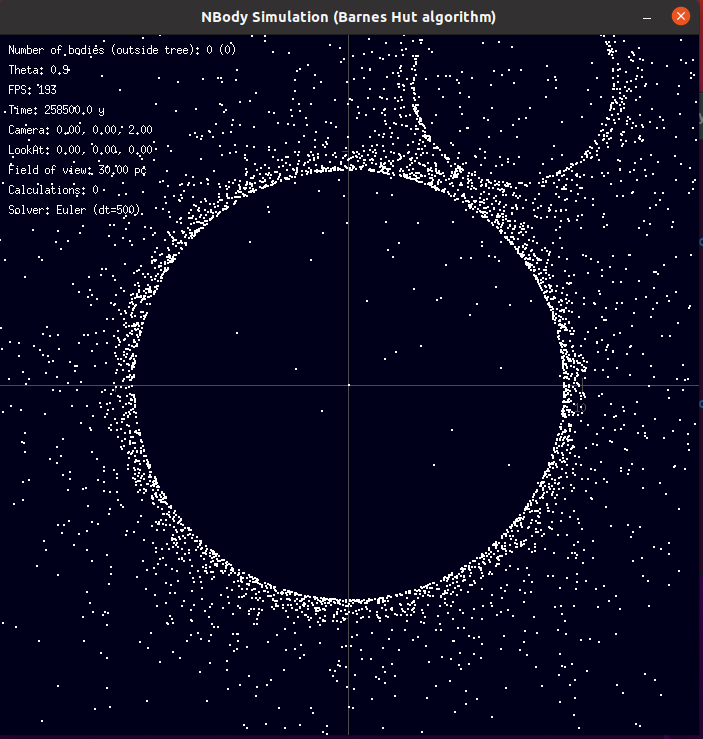
\includegraphics[width=13cm]{aff.png}
\end{center}
%légende de l'image
\caption{Visualisation (aucun calcul effectué)}
\end{figure}
 
